% !TEX root =  ../supplementary.tex
\section{Risk Predictions for Upgrading}
\label{sec:param_estimates_jm_fit_prias}
Let us assume a new patient $j$, for whom we need to estimate the upgrading-risk. Let his current follow-up visit time be $v$, latest time of biopsy be $t$, observed vector PSA measurements be $\mathcal{Y}_{j}(v)$. The combined information from the observed data about the time of upgrading, is given by the following posterior predictive distribution $g(T^*_j)$ of his time $T^*_j$ of upgrading:
\begin{equation*}
\label{eq:post_pred_dist}
\begin{aligned}
g(T^*_j) &= p\big\{T^*_j \mid T^*_j > t, \mathcal{Y}_{j}(v), \mathcal{A}_n\big\}\\
&= \int \int p\big(T^*_j \mid T^*_j > t, \boldsymbol{b}_j, \boldsymbol{\theta}\big) p\big\{\boldsymbol{b}_j \mid T^*_j>t, \mathcal{Y}_{j}(v), \boldsymbol{\theta}\big\}p\big(\boldsymbol{\theta} \mid \mathcal{A}_n\big) \mathrm{d} \boldsymbol{b}_j \mathrm{d} \boldsymbol{\theta}.
\end{aligned}
\end{equation*}
The distribution $g(T^*_j)$ depends not only depends on the observed data of the patient $T^*_j > t, \mathcal{Y}_{j}(v)$, but also depends on the information from the PRIAS dataset $\mathcal{A}_n$. To this the the posterior distribution of random effects $\boldsymbol{b}_j$ and posterior distribution of the vector of all parameters $\boldsymbol{\theta}$ are utilized, respectively. The distribution $g(T^*_j)$ can be estimated as detailed in \citet{rizopoulos2017dynamic}. Since, many prostate cancer patients may not obtain upgrading in the current follow-up period of PRIAS, $g(T^*_j)$ can only be estimated for a currently limited follow-up period.

The cause-specific cumulative upgrading-risk can be derived from $g(T^*_j)$ as given in~\citep{rizopoulos2017dynamic}. It is given by:
\begin{equation}
\label{eq:dynamic_risk_prob}
R_j(u \mid t, v) = \mbox{Pr}\big\{T^*_j > u \mid T^*_j > t, \mathcal{Y}_{j}(v), \mathcal{A}_n\big\}, \quad u \geq t.
\end{equation}
The personalized risk profile of the patient (see Panel~C, Figure~\ref{fig:dynrisk_plot_102}) updates as more data is gathered over follow-up visits. 

\begin{figure}
\centerline{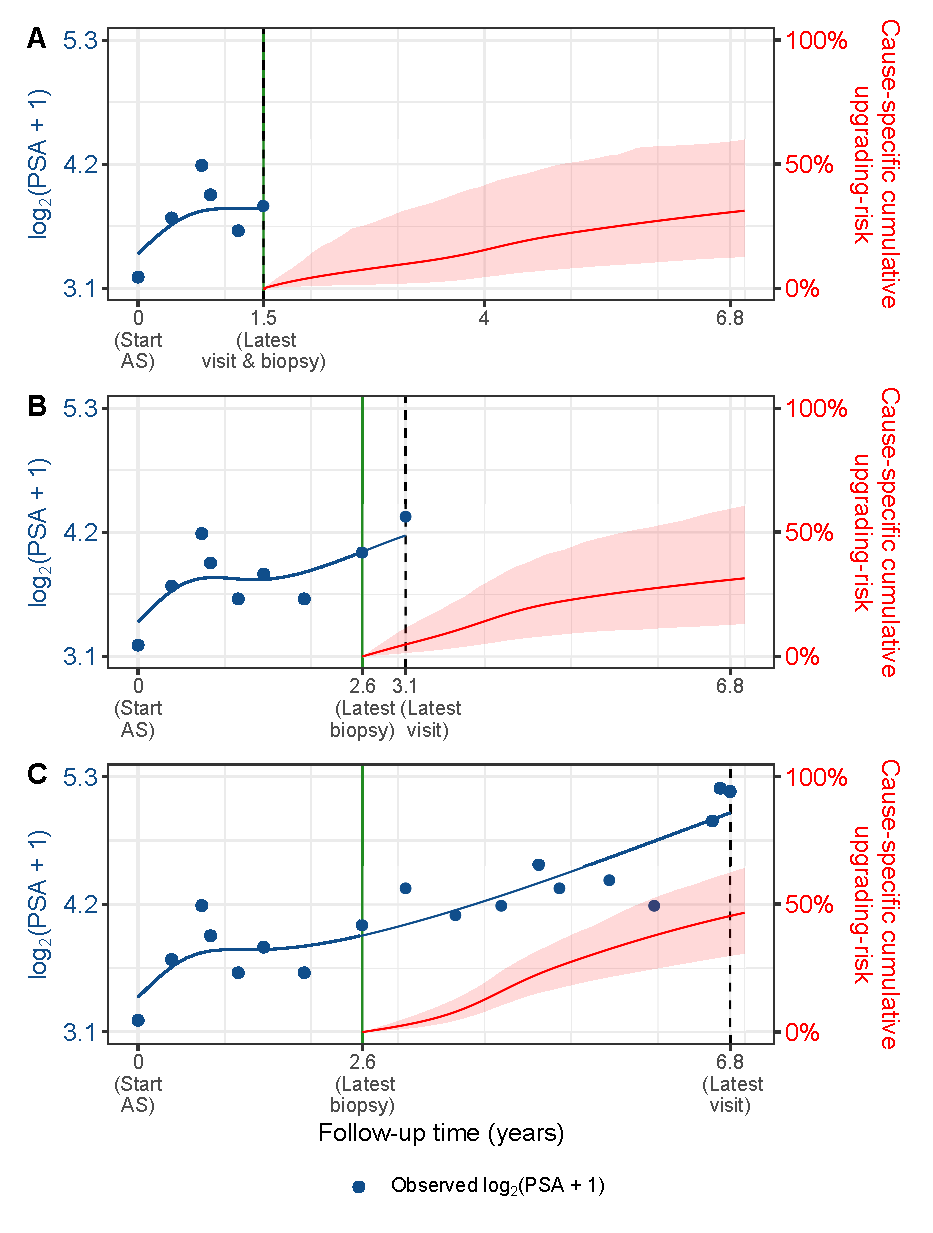
\includegraphics[width=\columnwidth]{images/dynrisk_plot_102.eps}}
\caption{\textbf{Cause-specific cumulative upgrading-risk changing dynamically over follow-up} as more patient data is gathered. The three \textbf{Panels~A,B~and~C:} are ordered by the time of the latest visit (dashed vertical black line) of a new patient. At each of the latest follow-up visits, we combine the accumulated PSA measurements (shown in blue), and latest time of negative biopsy (solid vertical green line) to obtain the updated cumulative-risk profile (shown in red) of the patient.}
\label{fig:dynrisk_plot_102}
\end{figure}

\clearpage
\subsection{Validation of Risk Predictions}
We wanted to check the usefulness of our model for not only the PRIAS patients but also for patients from other cohorts. To this end, we validated our model in the PRIAS dataset (internal validation) and the largest six cohorts from the GAP3 database~\citep{gap3_2018}. These are the University of Toronto AS (Toronto), Johns Hopkins AS (Hopkins), Memorial Sloan Kettering Cancer Center AS (MSKCC), University of California San Francisco Active Surveillance (UCSF), King's College London AS (KCL), Michigan Urological Surgery Improvement Collaborative AS (MUSIC).

\textbf{\textit{Calibration-in-the-large}}
We first assessed calibration-in-the-large~\citep{steyerberg2010assessing} of our model in the aforementioned cohorts. To this end, we used our model to predict the cause-specific cumulative upgrading-risk for each patient, given their PSA measurements and biopsy results. We then averaged the resulting profiles of cause-specific cumulative upgrading-risk. Subsequently, we compared the averaged cumulative-risk profile with a non-parametric estimate~\citep{turnbull1976empirical} of the cause-specific cumulative upgrading-risk in each of the cohorts. The results are shown in Panel~A of Figure~\ref{fig:calib_before_after}. We can see that our model is miscalibrated in external cohorts, although it is fine in the Hopkins cohort. To improve our model's calibration in all cohorts, we recalibrated the baseline hazard of the joint model fitted to the PRIAS dataset, individually for each of the cohorts except the Hopkins cohort. More specifically, given the data of an external cohort $\mathcal{A}^c$, where $c$ denotes the cohort, the recalibrated parameters $\boldsymbol{\gamma}_{h_0}^c$ (\ref{sec:jm_framework}) of the log baseline hazard are given by:
\begin{equation}
p(\boldsymbol{\gamma}_{h_0}^c \mid \mathcal{A}^c, \boldsymbol{b^c},  \boldsymbol{\theta}) \propto  \prod_{i=1}^{n^c} p(l_i^c, r_i^c \mid \boldsymbol{b^c_i}, \boldsymbol{\theta}) p(\boldsymbol{\gamma}_{h_0}^c)
\end{equation}
where $n^c$ are the number of patients in the $c$-th cohort, and $\boldsymbol{\theta}$ is the vector of all parameters of the joint model fitted to the PRIAS dataset. The interval in which upgrading is observed for the $i$-th patient is given by $l_i^c, r_i^c$, with $r_i^c = \infty$ for right-censored patients. The symbol $\boldsymbol{b^c_i}$ denotes patient-specific random effects (\ref{sec:jm_framework}) in the $c$-th cohort. The random effects are obtained using the joint model fitted to the PRIAS dataset before recalibration. We re-evaluated the calibration-in-the-large of our model after the recalibration of the baseline hazard individually for each cohort. The improved calibration-in-the-large is shown in Panel~B of Figure~\ref{fig:calib_before_after}.

\begin{figure}[!htb]
\centerline{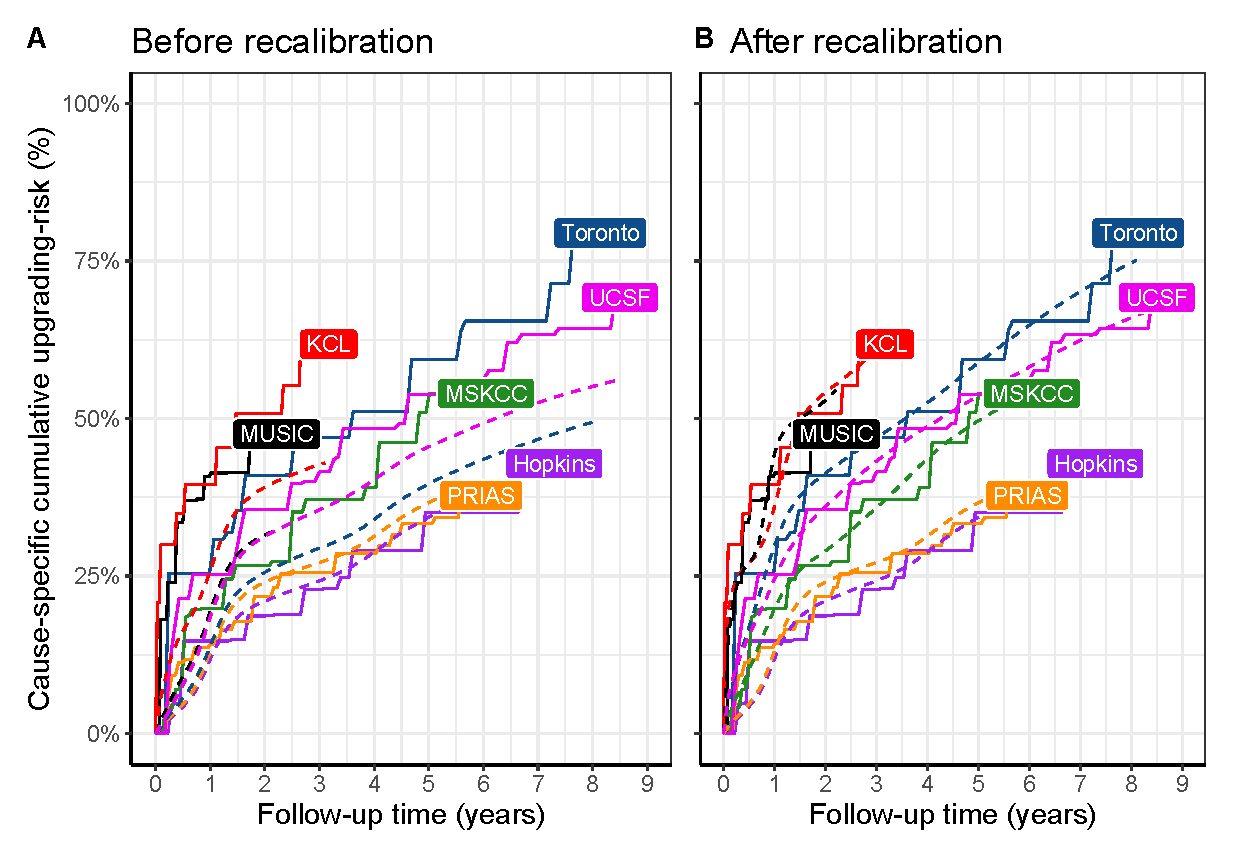
\includegraphics[width=\columnwidth]{images/calib_before_after.eps}}
\caption{\textbf{Calibration-in-the-large of our model:}. In \textbf{Panel~A} we can see that our model is not well calibrated for use in KCL, MUSIC, Toronto and MSKCC. In \textbf{Panel~B} we can see that calibration of model predictions improved in KCL, MUSIC, Toronto and MSKCC cohorts after recalibrating our model. Recalibration was not necessary for Hopkins cohort. Full names of Cohorts are \textit{PRIAS}: Prostate Cancer International Active Surveillance, \textit{Toronto}: University of Toronto Active Surveillance, \textit{Hopkins}: Johns Hopkins Active Surveillance, \textit{MSKCC}: Memorial Sloan Kettering Cancer Center Active Surveillance, \textit{KCL}: King's College London Active Surveillance, \textit{MUSIC}: Michigan Urological Surgery Improvement Collaborative Active Surveillance, \textit{UCSF}: University of California San Francisco Active Surveillance.}
\label{fig:calib_before_after}
\end{figure}

\clearpage
\textbf{\textit{Recalibrated PRIAS Model Versus Individual Joint Models For Each Cohort}}
We wanted to check if our recalibrated PRIAS model performed as good as a new joint model that could be fitted to the external cohorts. To this end, we predicted cause-specific cumulative upgrading-risk for each patient from each cohort using two sets of models, namely the recalibrated PRIAS model for each cohort, and a new joint model fitted to each cohort. The difference in predicted cause-specific cumulative upgrading-risk from these models is shown in Figure~\ref{fig:calib_insmall_after}. We can see that the difference is smaller in those cohorts in which the effects of $\log_2 (\mbox{PSA} + 1)$ value and velocity were similar to that of PRIAS~(Table~\ref{tab:PSA_survival_gap3}). For example, the Hopkins cohort had parameter estimates similar to that of PRIAS, and consequently, the difference in predicted risks for this cohort is smallest. The opposite of this phenomenon holds for the MUSIC and KCL cohorts.
 
\begin{figure}[!htb]
\centerline{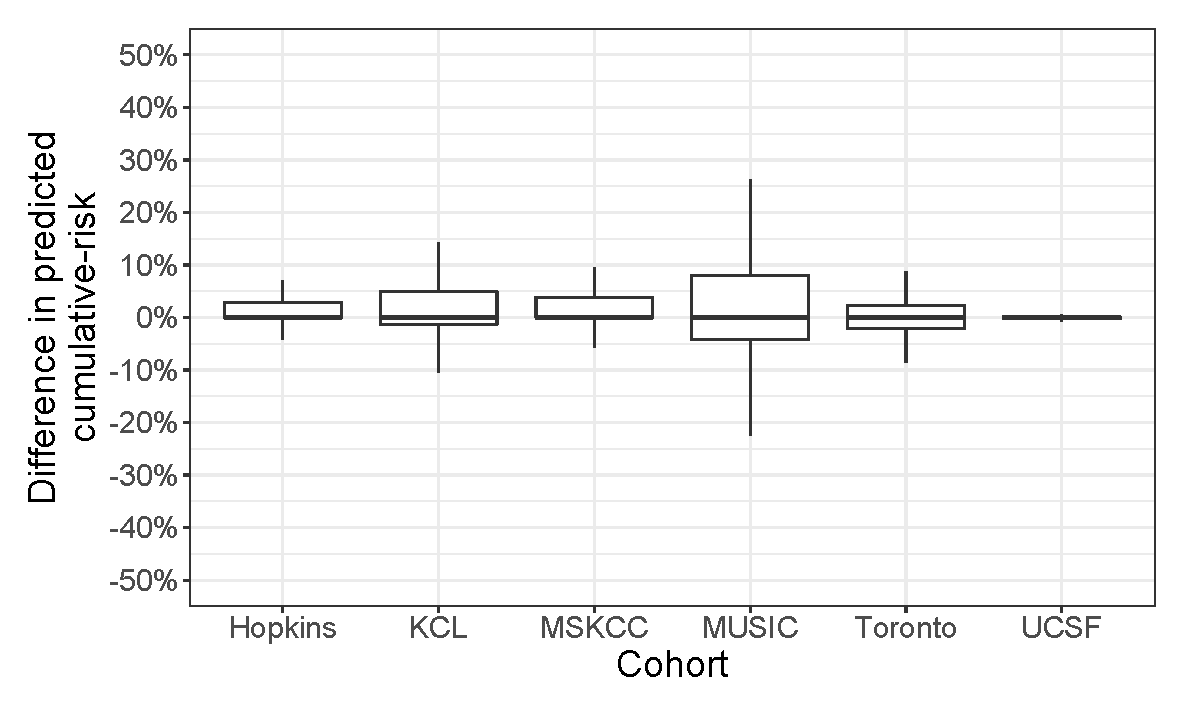
\includegraphics[width=0.85\columnwidth]{images/calib_insmall_after.eps}}
\caption{\textbf{Comparison of predictions from recalibrated PRIAS model with individual joint models fitted to external cohorts:} On Y-axis we show the difference between predicted cause-specific cumulative upgrading-risk for individual patients using two models, namely the recalibrated PRIAS model for each cohort, and individual joint model fitted to each cohort. The figure shows that the difference is smaller in those cohorts in which the effects of $\log_2 (\mbox{PSA} + 1)$ value and velocity were similar to that of PRIAS~(Table~\ref{tab:PSA_survival_gap3}). Full names of Cohorts are \textit{PRIAS}: Prostate Cancer International Active Surveillance, \textit{Toronto}: University of Toronto Active Surveillance, \textit{Hopkins}: Johns Hopkins Active Surveillance, \textit{MSKCC}: Memorial Sloan Kettering Cancer Center Active Surveillance, \textit{KCL}: King's College London Active Surveillance, \textit{MUSIC}: Michigan Urological Surgery Improvement Collaborative Active Surveillance, \textit{UCSF}: University of California San Francisco Active Surveillance.}
\label{fig:calib_insmall_after}
\end{figure}

\clearpage
\textbf{\textit{Validation of Dynamic Cumulative-Risk Predictions}}
As shown in Figure~\ref{fig:dynrisk_plot_102}, the cumulative-risk predictions from the joint model are dynamic in nature. That is, they update as more data becomes available over time. Consequently, the discrimination and prediction error of the joint model also depend on the available data. We assessed these two measures dynamically in the PRIAS cohort (interval validation) and in the largest six external cohorts that are part of the GAP3 database. For discrimination, we utilized the time-varying area under the receiver operating characteristic curve or time-varying AUC~\citep{rizopoulos2017dynamic}. For time-varying prediction error, we assessed the mean absolute prediction error or MAPE~\citep{rizopoulos2017dynamic}. The AUC indicates how well the model discriminates between patients who experience upgrading, and those do not. The MAPE indicates how accurately the model predicts upgrading. Both AUC and MAPE are restricted to $[0,1]$. However, it is preferred that AUC $>$ 0.5 because an AUC $\leq$ 0.5 indicates that the model performs worse than random discrimination. Ideally, MAPE should be 0.

We calculate AUC and MAPE in a time-dependent manner. More specifically, given the time of latest biopsy $t$, and history of PSA measurements up to time $v$, we calculate AUC and MAPE for a medically relevant time frame $(t, v]$, within which the occurrence of upgrading is of interest. In the case of prostate cancer, at any point in time $v$, it is of interest to identify patients who may have experienced upgrading in the last one year $(v-1, v]$. That is, we set $t=v-1$. We then calculate AUC and MAPE at a gap of every six months (follow-up schedule of PRIAS). That is, $v \epsilon \{1, 1.5, \ldots \}$ years. To obtain reliable estimates of AUC and MAPE, in each cohort, we restrict $v$ to a maximum time point $v_{\mbox{max}}$, such that there are at least ten patients who experience upgrading after $v_{\mbox{max}}$. This maximum time point $v_{\mbox{max}}$ differs between cohorts, and is given in Table~\ref{tab:max_pred_time}.

\begin{table}[!htb]
\small\sf\centering
\caption{\textbf{Maximum follow-up period up to which we can reliably predict upgrading-risk}. In each cohort, this time point is chosen such that there are at least 10 patients who experience upgrading after this time point. Full names of Cohorts are \textit{PRIAS}: Prostate Cancer International Active Surveillance, \textit{Toronto}: University of Toronto Active Surveillance, \textit{Hopkins}: Johns Hopkins Active Surveillance, \textit{MSKCC}: Memorial Sloan Kettering Cancer Center Active Surveillance, \textit{KCL}: King's College London Active Surveillance, \textit{MUSIC}: Michigan Urological Surgery Improvement Collaborative Active Surveillance, \textit{UCSF}: University of California San Francisco Active Surveillance.}
\label{tab:max_pred_time}
\begin{tabular}{l|r}
\hline
\hline
Cohort & \parbox[t]{3.5cm}{Maximum Prediction\\Time (years)}\\
\hline
PRIAS & 6\\
KCL & 3\\
MUSIC & 2\\
Toronto & 8\\
MSKCC & 6\\
Hopkins & 7\\
UCSF & 8.5\\
\hline
\end{tabular}    
\end{table}

The results for estimates of AUC and MAPE are summarized in Figure~\ref{fig:auc_pe_recalib}, and in Table~\ref{tab:AUC_PE_PRIAS} to Table~\ref{tab:AUC_PE_MUSIC}. Results are based on the recalibrated PRIAS model for the GAP3 cohorts. The results show that AUC remains more or less constant in all cohorts as more data becomes available for patients. The AUC obtains a moderate value, roughly between 0.5 and 0.7 for all cohorts. On the other hand, MAPE reduces by a big margin after year one of follow-up. This could be because of two reasons. Firstly, MAPE at year one is based only on four PSA measurements gathered in the first year of follow-up, whereas after year one number of PSA measurements increases. Secondly, patients in year one consist of two sub-populations, namely patients with a correct Gleason grade group~1 at the time of inclusion in AS, and patients who probably had Gleason grade group~2 at inclusion but were misclassified by the urologist as Gleason grade group~1 patients. To remedy this problem, a biopsy for all patients at year one is commonly recommended in all AS programs~\citep{bokhorst2015compliance}.

\begin{figure}[!htb]
\centerline{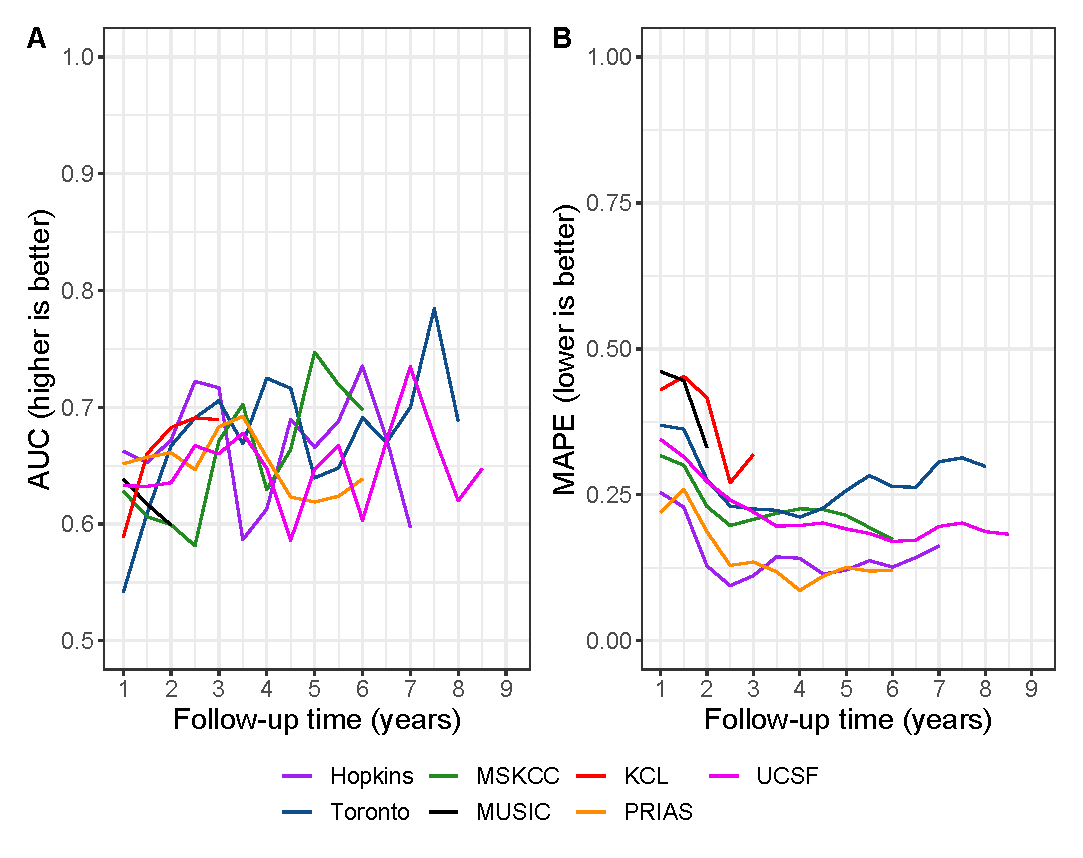
\includegraphics[width=\columnwidth]{images/auc_pe_recalib.eps}}
\caption{\textbf{Validation of dynamic predictions of cause-specific cumulative upgrading-risk}. In \textbf{Panel~A} we can see that the time dependent area under the receiver operating characteristic curve or AUC (measure of discrimination) is above 0.5 in PRIAS (internal validation), and in Toronto, Hopkins, MSKCC, KCL, and MUSIC AS cohorts (external validation). In \textbf{Panel~B} we can see that the time dependent root mean squared prediction error or MAPE is similar for PRIAS and Hopkins cohorts. The bootstrapped 95\% confidence interval for these estimates are presented in Table~\ref{tab:AUC_PE_PRIAS} to Table~\ref{tab:AUC_PE_KCL}. Full names of Cohorts are \textit{PRIAS}: Prostate Cancer International Active Surveillance, \textit{Toronto}: University of Toronto Active Surveillance, \textit{Hopkins}: Johns Hopkins Active Surveillance, \textit{MSKCC}: Memorial Sloan Kettering Cancer Center Active Surveillance, \textit{KCL}: King's College London Active Surveillance, \textit{MUSIC}: Michigan Urological Surgery Improvement Collaborative Active Surveillance, \textit{UCSF}: University of California San Francisco Active Surveillance.}
\label{fig:auc_pe_recalib}
\end{figure}

\begin{table}[!htb]
\small\sf\centering
\caption{\textbf{Internal validation of predictions of upgrading in PRIAS cohort}. The area under the receiver operating characteristic curve or AUC (measure of discrimination) and mean absolute prediction error or MAPE are calculated over the follow-up period at a gap of 6 months. In addition bootstrapped 95\% confidence intervals (CI) are also presented.}
\label{tab:AUC_PE_PRIAS}
\begin{tabular}{r|r|r}
\hline
\hline
Follow-up period (years) & AUC (95\% CI) & MAPE (95\%CI)\\ 
\hline
0.0 to 1.0 & 0.652 [0.611, 0.690] & 0.220 [0.214, 0.227]\\
0.5 to 1.5 & 0.657 [0.641, 0.673] & 0.260 [0.254, 0.265]\\
1.0 to 2.0 & 0.661 [0.647, 0.678] & 0.187 [0.183, 0.191]\\
1.5 to 2.5 & 0.647 [0.596, 0.688] & 0.129 [0.122, 0.140]\\
2.0 to 3.0 & 0.683 [0.642, 0.723] & 0.135 [0.125, 0.146]\\
2.5 to 3.5 & 0.692 [0.632, 0.748] & 0.118 [0.111, 0.128]\\
3.0 to 4.0 & 0.657 [0.603, 0.709] & 0.086 [0.080, 0.092]\\
3.5 to 4.5 & 0.623 [0.582, 0.660] & 0.111 [0.105, 0.116]\\
4.0 to 5.0 & 0.619 [0.582, 0.654] & 0.126 [0.118, 0.131]\\
4.5 to 5.5 & 0.624 [0.537, 0.711] & 0.119 [0.103, 0.135]\\
5.0 to 6.0 & 0.639 [0.582, 0.696] & 0.121 [0.103, 0.138]\\
\hline
\end{tabular}    
\end{table}

\begin{table}[!htb]
\small\sf\centering
\caption{\textbf{External validation of predictions of upgrading in University of Toronto Active Surveillance cohort}. The area under the receiver operating characteristic curve or AUC (measure of discrimination) and mean absolute prediction error or MAPE are calculated over the follow-up period at a gap of 6 months. In addition bootstrapped 95\% confidence intervals (CI) are also presented.}
\label{tab:AUC_PE_Toronto}
\begin{tabular}{r|r|r}
\hline
\hline
Follow-up period (years) & AUC (95\% CI) & MAPE (95\%CI)\\ 
\hline
0.0 to 1.0 & 0.541 [0.470, 0.621] & 0.369 [0.352, 0.381]\\
0.5 to 1.5 & 0.609 [0.547, 0.661] & 0.363 [0.348, 0.376]\\
1.0 to 2.0 & 0.667 [0.634, 0.712] & 0.276 [0.259, 0.296]\\
1.5 to 2.5 & 0.691 [0.651, 0.730] & 0.231 [0.205, 0.254]\\
2.0 to 3.0 & 0.706 [0.637, 0.762] & 0.226 [0.196, 0.260]\\
2.5 to 3.5 & 0.669 [0.586, 0.741] & 0.224 [0.195, 0.258]\\
3.0 to 4.0 & 0.725 [0.649, 0.806] & 0.212 [0.184, 0.238]\\
3.5 to 4.5 & 0.716 [0.642, 0.793] & 0.227 [0.206, 0.258]\\
4.0 to 5.0 & 0.640 [0.579, 0.717] & 0.257 [0.222, 0.312]\\
4.5 to 5.5 & 0.648 [0.579, 0.740] & 0.283 [0.247, 0.326]\\
5.0 to 6.0 & 0.691 [0.608, 0.793] & 0.264 [0.232, 0.302]\\
5.5 to 6.5 & 0.670 [0.543, 0.776] & 0.263 [0.227, 0.307]\\
6.0 to 7.0 & 0.700 [0.544, 0.851] & 0.307 [0.258, 0.363]\\
6.5 to 7.5 & 0.785 [0.640, 0.866] & 0.313 [0.272, 0.360]\\
7.0 to 8.0 & 0.688 [0.532, 0.786] & 0.299 [0.249, 0.361]\\
\hline
\end{tabular}    
\end{table}

\begin{table}[!htb]
\small\sf\centering
\caption{\textbf{External validation of predictions of upgrading in University of California San Francisco Active Surveillance cohort}. The area under the receiver operating characteristic curve or AUC (measure of discrimination) and mean absolute prediction error or MAPE are calculated over the follow-up period at a gap of 6 months. In addition bootstrapped 95\% confidence intervals (CI) are also presented.}
\label{tab:AUC_PE_UCSF}
\begin{tabular}{r|r|r}
\hline
\hline
Follow-up period (years) & AUC (95\% CI) & MAPE (95\%CI)\\ 
\hline
0.0 to 1.0 & 0.633 [0.585, 0.674] & 0.345 [0.337, 0.357]\\
0.5 to 1.5 & 0.632 [0.599, 0.673] & 0.315 [0.308, 0.323]\\
1.0 to 2.0 & 0.635 [0.595, 0.677] & 0.273 [0.266, 0.281]\\
1.5 to 2.5 & 0.667 [0.628, 0.715] & 0.241 [0.224, 0.259]\\
2.0 to 3.0 & 0.660 [0.600, 0.713] & 0.221 [0.205, 0.238]\\
2.5 to 3.5 & 0.678 [0.614, 0.757] & 0.197 [0.175, 0.214]\\
3.0 to 4.0 & 0.648 [0.574, 0.707] & 0.197 [0.179, 0.221]\\
3.5 to 4.5 & 0.586 [0.525, 0.638] & 0.202 [0.180, 0.229]\\
4.0 to 5.0 & 0.647 [0.590, 0.754] & 0.192 [0.168, 0.217]\\
4.5 to 5.5 & 0.667 [0.582, 0.773] & 0.184 [0.159, 0.220]\\
5.0 to 6.0 & 0.603 [0.496, 0.696] & 0.170 [0.144, 0.207]\\
5.5 to 6.5 & 0.671 [0.576, 0.786] & 0.173 [0.145, 0.202]\\
6.0 to 7.0 & 0.735 [0.663, 0.794] & 0.196 [0.166, 0.219]\\
6.5 to 7.5 & 0.675 [0.565, 0.769] & 0.202 [0.168, 0.231]\\
7.0 to 8.0 & 0.620 [0.518, 0.740] & 0.187 [0.144, 0.217]\\
7.5 to 8.5 & 0.647 [0.538, 0.787] & 0.183 [0.146, 0.222]\\
\hline
\end{tabular}    
\end{table}

\begin{table}[!htb]
\small\sf\centering
\caption{\textbf{External validation of predictions of upgrading in Johns Hopkins Active Surveillance cohort}. The area under the receiver operating characteristic curve or AUC (measure of discrimination) and mean absolute prediction error or MAPE are calculated over the follow-up period at a gap of 6 months. In addition bootstrapped 95\% confidence intervals (CI) are also presented.}
\label{tab:AUC_PE_Hopkins}
\begin{tabular}{r|r|r}
\hline
\hline
Follow-up period (years) & AUC (95\% CI) & MAPE (95\%CI)\\ 
\hline
0.0 to 1.0 & 0.662 [0.586, 0.715] & 0.254 [0.245, 0.265]\\
0.5 to 1.5 & 0.653 [0.603, 0.707] & 0.229 [0.219, 0.240]\\
1.0 to 2.0 & 0.672 [0.604, 0.744] & 0.128 [0.115, 0.141]\\
1.5 to 2.5 & 0.722 [0.652, 0.792] & 0.095 [0.081, 0.111]\\
2.0 to 3.0 & 0.717 [0.638, 0.777] & 0.112 [0.100, 0.123]\\
2.5 to 3.5 & 0.587 [0.493, 0.704] & 0.144 [0.129, 0.154]\\
3.0 to 4.0 & 0.613 [0.486, 0.742] & 0.141 [0.126, 0.156]\\
3.5 to 4.5 & 0.690 [0.594, 0.783] & 0.115 [0.100, 0.133]\\
4.0 to 5.0 & 0.666 [0.572, 0.754] & 0.121 [0.104, 0.147]\\
4.5 to 5.5 & 0.688 [0.519, 0.779] & 0.137 [0.119, 0.161]\\
5.0 to 6.0 & 0.735 [0.676, 0.820] & 0.126 [0.102, 0.152]\\
5.5 to 6.5 & 0.674 [0.581, 0.765] & 0.143 [0.121, 0.172]\\
6.0 to 7.0 & 0.597 [0.472, 0.712] & 0.163 [0.126, 0.195]\\
\hline
\end{tabular}    
\end{table}

\begin{table}[!htb]
\small\sf\centering
\caption{\textbf{External validation of predictions of upgrading in Memorial Sloan Kettering Cancer Center Active Surveillance cohort}. The area under the receiver operating characteristic curve or AUC (measure of discrimination) and mean absolute prediction error or MAPE are calculated over the follow-up period at a gap of 6 months. In addition bootstrapped 95\% confidence intervals (CI) are also presented.}
\label{tab:AUC_PE_MSKCC}
\begin{tabular}{r|r|r}
\hline
\hline
Follow-up period (years) & AUC (95\% CI) & MAPE (95\%CI)\\ 
\hline
0.0 to 1.0 & 0.628 [0.577, 0.688]  & 0.317 [0.316, 0.318]\\
0.5 to 1.5 & 0.606 [0.532, 0.657]  & 0.301 [0.290, 0.311]\\
1.0 to 2.0 & 0.599 [0.518, 0.671]  & 0.230 [0.207, 0.256]\\
1.5 to 2.5 & 0.581 [0.504, 0.663]  & 0.198 [0.168, 0.235]\\
2.0 to 3.0 & 0.671 [0.599, 0.741]  & 0.208 [0.182, 0.232]\\
2.5 to 3.5 & 0.703 [0.610, 0.777]  & 0.218 [0.197, 0.246]\\
3.0 to 4.0 & 0.629 [0.499, 0.706]  & 0.226 [0.194, 0.259]\\
3.5 to 4.5 & 0.664 [0.589, 0.756]  & 0.225 [0.199, 0.262]\\
4.0 to 5.0 & 0.747 [0.642, 0.841]  & 0.215 [0.188, 0.247]\\
4.5 to 5.5 & 0.719 [0.597, 0.852]  & 0.194 [0.165, 0.232]\\
5.0 to 6.0 & 0.698 [0.565, 0.792]  & 0.174 [0.136, 0.227]\\
\hline
\end{tabular}    
\end{table}

\begin{table}[!htb]
\small\sf\centering
\caption{\textbf{External validation of predictions of upgrading in King's College London Active Surveillance cohort}. The area under the receiver operating characteristic curve or AUC (measure of discrimination) and mean absolute prediction error or MAPE are calculated over the follow-up period at a gap of 6 months. In addition bootstrapped 95\% confidence intervals (CI) are also presented.}
\label{tab:AUC_PE_KCL}
\begin{tabular}{r|r|r}
\hline
\hline
Follow-up period (years) & AUC (95\% CI) & MAPE (95\%CI)\\ 
\hline
0.0 to 1.0 & 0.589 [0.514, 0.653] & 0.430 [0.407, 0.450] \\
0.5 to 1.5 & 0.660 [0.550, 0.742] & 0.453 [0.431, 0.474] \\
1.0 to 2.0 & 0.683 [0.604, 0.753] & 0.416 [0.396, 0.445] \\
1.5 to 2.5 & 0.691 [0.621, 0.766] & 0.271 [0.246, 0.297] \\
2.0 to 3.0 & 0.689 [0.616, 0.785] & 0.319 [0.282, 0.344] \\
\hline
\end{tabular}    
\end{table}

\begin{table}[!htb]
\small\sf\centering
\caption{\textbf{External validation of predictions of upgrading in Michigan Urological Surgery Improvement Collaborative Active Surveillance cohort}. The area under the receiver operating characteristic curve or AUC (measure of discrimination) and mean absolute prediction error or MAPE are calculated over the follow-up period at a gap of 6 months. In addition bootstrapped 95\% confidence intervals (CI) are also presented.}
\label{tab:AUC_PE_MUSIC}
\begin{tabular}{r|r|r}
\hline
\hline
Follow-up period (years) & AUC (95\% CI) & MAPE (95\%CI)\\ 
\hline
0.0 to 1.0 & 0.639 [0.607, 0.672] & 0.461 [0.450, 0.469]\\
0.5 to 1.5 & 0.617 [0.588, 0.652] & 0.446 [0.441, 0.453]\\
1.0 to 2.0 & 0.599 [0.553, 0.632] & 0.331 [0.317, 0.348]\\
\hline
\end{tabular}    
\end{table}